% !TEX root = ../thesis.tex

\chapter{Case Study I: Building Health Monitoring} \label{chp:building}

\section{Domain and Experimental Objectives}

Building health monitoring represents a critical application domain for L1 Descriptive Twin validation, providing an ideal environment for testing DT-RAG capabilities and information fusion approaches. This domain involves complex data integration challenges typical of modern cyber-physical systems while maintaining manageable complexity for systematic evaluation.

Modern building management systems generate vast amounts of heterogeneous data from IoT sensors, Building Information Models (BIM), maintenance records, and operational documentation. This data diversity creates ideal conditions for testing the CORTEX Perception Module's ability to integrate and reason about multi-modal information sources. The building domain provides clear diagnostic objectives with verifiable ground truth, enabling rigorous evaluation of cognitive enhancement benefits.

The experimental setup focuses on fault detection and diagnosis tasks that require reasoning across multiple information sources. Unlike simple threshold-based monitoring systems, effective building diagnosis requires understanding complex relationships between symptoms, potential causes, and system interdependencies. This cognitive complexity makes the domain particularly suitable for demonstrating the value of LLM-enhanced approaches over traditional rule-based systems.


Traditional approaches to building monitoring typically rely on simple threshold-based alerts and isolated sensor analysis. These approaches suffer from high false positive rates due to their inability to consider system context and interdependencies. For example, a temperature sensor reading may appear anomalous in isolation but be completely normal when considered alongside HVAC schedules, occupancy patterns, and weather conditions.

Direct application of LLMs without proper grounding mechanisms reveals several critical limitations. LLMs lack access to real-time sensor data and cannot query structured databases containing historical information. They demonstrate poor understanding of temporal relationships in building operations and show inconsistent reasoning about physical cause-and-effect relationships. Finally, they cannot access technical documentation and maintenance records that are crucial for accurate diagnosis.

The research objectives focus on demonstrating the effectiveness of DT-RAG in addressing these limitations through comprehensive data integration and contextual reasoning. Primary objectives include validating the ability to integrate heterogeneous data sources (BIM models, IoT sensors, maintenance records) into coherent reasoning contexts, demonstrating improved diagnostic accuracy compared to traditional threshold-based approaches, and quantifying the reduction in false positive rates through contextual reasoning.

Secondary objectives involve establishing performance baselines for information synthesis tasks, validating the scalability of the approach across different building types and systems, and developing reusable frameworks for similar infrastructure monitoring applications.

\section{Twin Construction and CORTEX Implementation}

Building upon the principles of comprehensive DT architecture, we implement a three-layer framework that enables sophisticated data management and real-time synchronization between physical buildings and their digital counterparts. This structure facilitates advanced monitoring, analysis, and decision-making in building defect management.

\begin{figure}[htbp]
\centering
\includegraphics[width=1\textwidth]{dt-framework.png}
\caption{A comprehensive DT architecture for building defect management, illustrating the three-layer structure: (1) Data Layer incorporating GeoBIM modeling, defect modeling, and expert knowledge integration, (2) DT Layer managing spatial information carriers, defect data schemas, and domain knowledge repositories, and (3) Decision Layer leveraging RAG and LLM techniques for advanced reasoning and human-in-the-loop decision-making.}
\label{fig:dt-framework-building}
\end{figure}

As shown in Fig.~\ref{fig:dt-framework-building}, the \textbf{Data Layer} incorporates three primary components: GeoBIM modeling, defect modeling, and expert knowledge integration. The GeoBIM modeling component combines multiple data sources, including 3D mesh models, BIM models, GIS information, and geo-AI knowledge bases. The defect modeling component processes aerial photographs of building facades, employing detection algorithms to identify RGB defects, infrared anomalies, and defect classifications. Expert knowledge integration leverages inspection reports, technical standards, legal frameworks, and defect manuals to enrich the defect data with domain-specific insights.

The \textbf{DT Layer} serves as the core of the digital representation, implementing three distinct data carriers to manage and organize the diverse information streams. Spatial information carriers handle formats such as IFC, RVT, and KML, ensuring proper management of spatial data and geometric relationships. Additionally, defect data schemas (XML, JSON, CSV, database) and domain knowledge repositories (PDF, DOCX, Markdown) provide standardized storage formats, ensuring seamless compatibility with the retrieval workflows.

The \textbf{Decision Layer} leverages retrieval augmented generation (RAG) and large language model (LLM) techniques for advanced reasoning and human-in-the-loop decision-making. By storing vector embeddings in databases, retrieving and reranking relevant chunks of domain-specific information, and routing user queries through AI-driven modules, this layer provides actionable insights in building defect management.

The building diagnosis task formalization establishes a systematic framework for evaluating diagnostic reasoning capabilities in complex infrastructure systems. The task requires identifying potential faults or anomalies in building systems based on comprehensive analysis of available data sources and providing explanatory reasoning that justifies diagnostic conclusions.

Formal problem definition: Given a building Digital Twin containing BIM data (B), sensor time series (S), maintenance records (M), and operational documentation (D), along with a natural language query describing symptoms or concerns (Q), generate a diagnostic assessment (A) that includes fault identification, confidence estimation, explanatory reasoning, and recommended actions.

\begin{figure}[htbp]
\centering
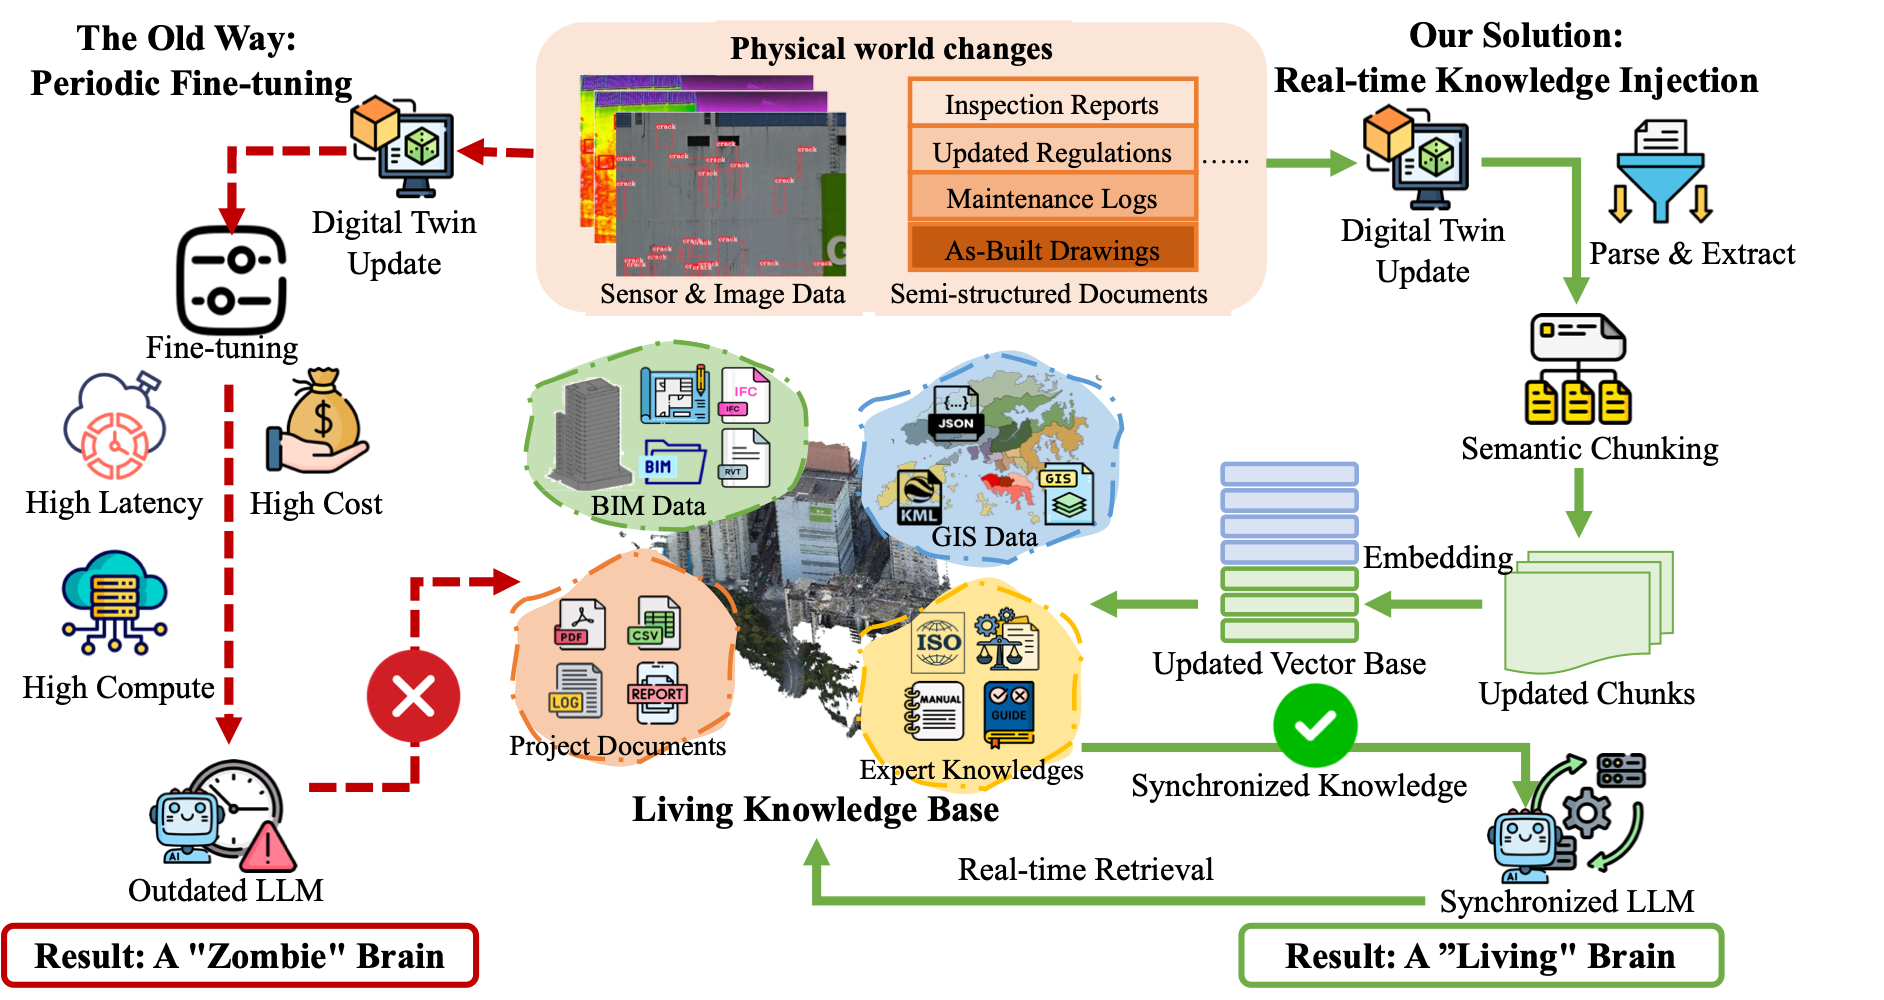
\includegraphics[width=0.9\textwidth]{DefectGPT/dynamic_knowledge_engine.png}
\caption{Dynamic knowledge engine architecture integrating real-time sensor data with historical building information models.}
\label{fig:dynamic_knowledge_engine}
\end{figure}

The solution approach must demonstrate capability for multi-source data integration, temporal reasoning about system behavior, causal analysis of potential fault mechanisms, and uncertainty quantification for diagnostic conclusions.



The L1 Descriptive Twin construction integrates multiple data sources into a comprehensive representation of building state and history. The core components include BIM geometric models providing spatial relationships, system layouts, and equipment specifications; sensor networks delivering real-time data on temperature, humidity, air quality, energy consumption, and occupancy; maintenance databases containing historical service records, warranty information, and replacement schedules; and operational documentation including system manuals, troubleshooting guides, and performance specifications.

Data preprocessing involves temporal alignment to synchronize data from different sources to common time references, spatial registration to map sensor locations to BIM geometric coordinates, quality assessment to identify and handle missing, corrupted, or anomalous data points, and semantic annotation to add contextual metadata that supports reasoning tasks.

The resulting Digital Twin provides a comprehensive, queryable representation of building state that serves as the foundation for cognitive reasoning tasks. This representation maintains real-time currency while preserving historical context necessary for effective diagnostic reasoning.

\begin{figure}[htbp]
\centering
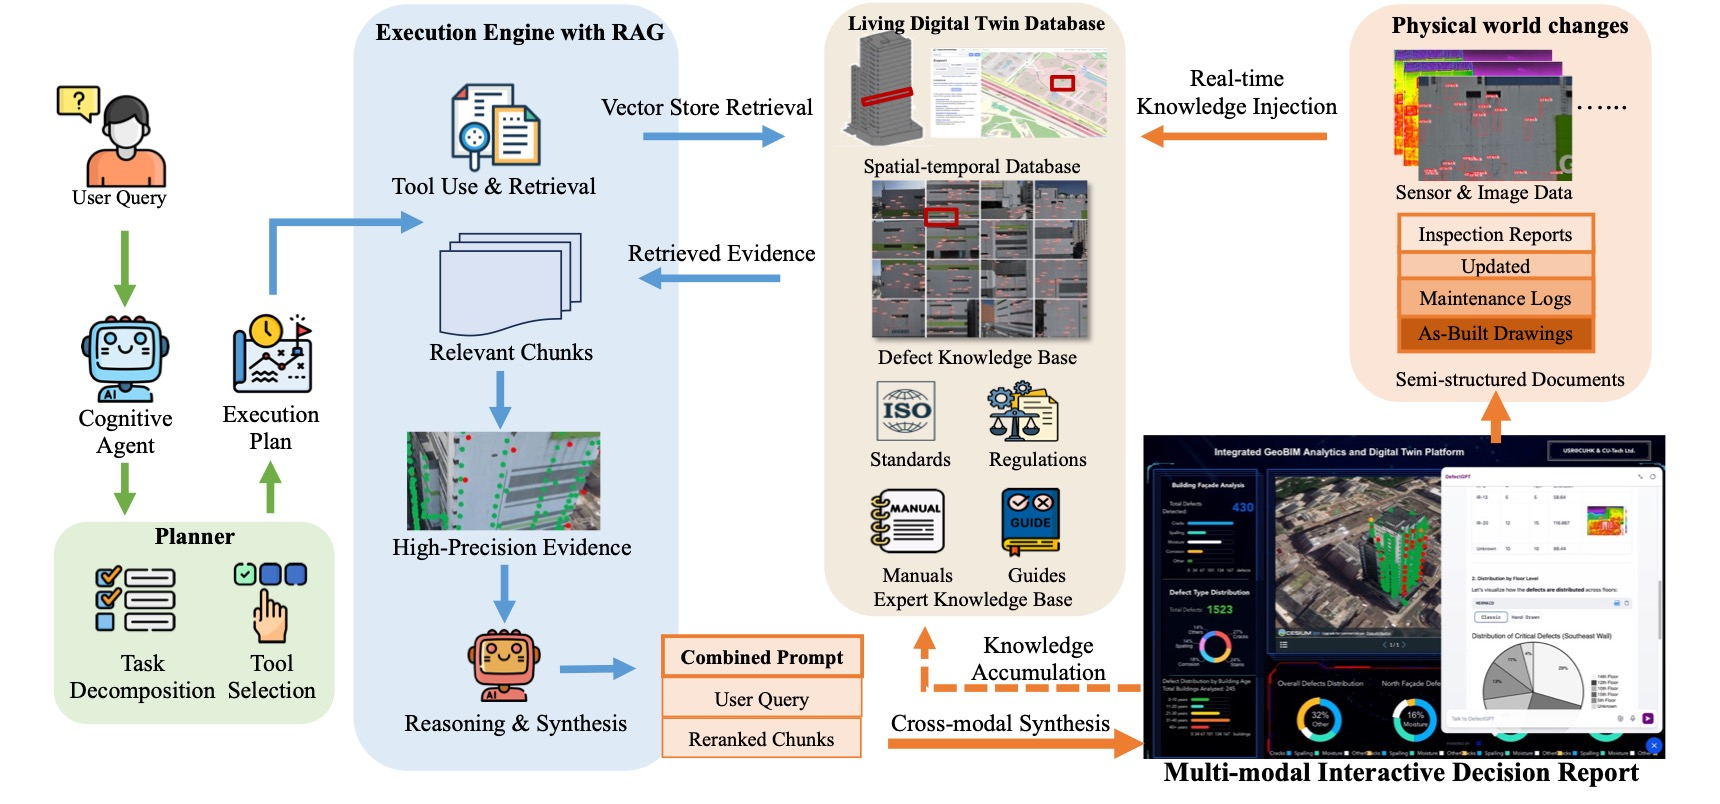
\includegraphics[width=0.9\textwidth]{figures/DefectGPT/cognitive_agent_framework.png}

\caption{The Cognitive Agent Framework showing the plan-retrieve-synthesize cognitive loop. The system processes queries through deliberate planning, targeted information retrieval, and comprehensive synthesis to generate diagnostic insights.}
\label{fig:cognitive_agent_framework}
\end{figure}

The CORTEX Perception Module implementation extends traditional RAG architectures to handle the heterogeneous, multi-modal data typical of building systems. The implementation includes specialized adapters for each data type, sophisticated fusion mechanisms for integrating results, and optimized summarization for LLM processing.

Task decomposition involves analyzing incoming diagnostic queries to identify the types of information needed for comprehensive assessment. The system decomposes complex queries into specific sub-tasks that can be addressed through targeted data retrieval operations. For example, a query about HVAC performance might be decomposed into sub-tasks addressing current sensor readings, historical performance trends, maintenance history, and system specifications.

The decomposition process considers temporal aspects (what time periods are relevant), spatial aspects (which building zones or systems are involved), and causal aspects (what potential failure mechanisms should be investigated). This systematic approach ensures comprehensive coverage while avoiding unnecessary computation.

The Hybrid Retrieval Engine implements parallel execution of specialized adapters designed for different data types. The SQL adapter generates and executes complex database queries to extract relevant information from structured databases containing BIM data, equipment specifications, and maintenance records. The time-series adapter handles specialized queries for temporal data including statistical analysis, trend detection, and anomaly identification. The vector search adapter performs semantic similarity searches across unstructured documents including manuals, reports, and troubleshooting guides.

\begin{figure}[htbp]
\centering
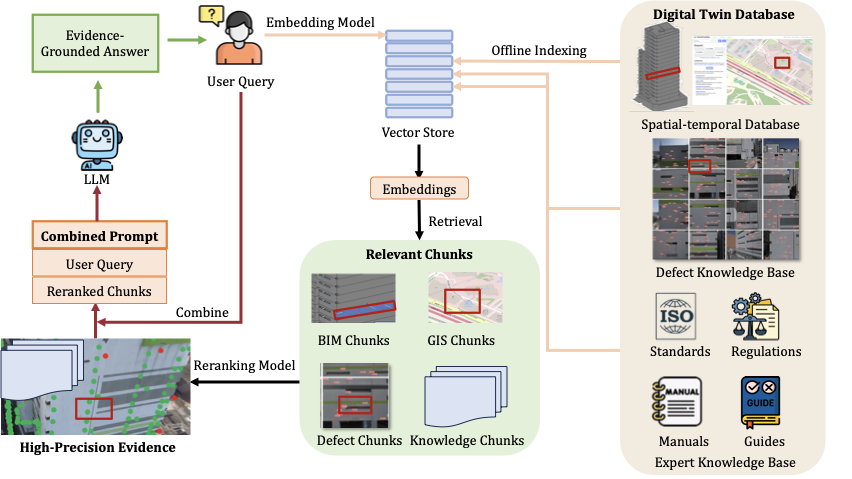
\includegraphics[width=0.9\textwidth]{DefectGPT/hybrid_retrieval_engine.png}

\caption{Hybrid retrieval engine demonstrating multi-modal data fusion from BIM geometric models, IoT sensor time-series, and technical documentation for comprehensive building diagnosis.}
\label{fig:hybrid_retrieval_engine}
\end{figure}

Result fusion represents the most critical component of the Perception Module, responsible for integrating heterogeneous information into coherent textual summaries optimized for LLM reasoning. The fusion process handles semantic alignment to ensure different data sources refer to the same physical entities, temporal coherence to present information in logical temporal sequences, and contextual prioritization to emphasize the most relevant information for the specific diagnostic task.

The fusion algorithm employs graph-based approaches to model relationships between different pieces of information, attention mechanisms to weight information importance, and template-based generation to produce structured summaries that preserve essential quantitative relationships while being optimized for natural language processing.

Reasoning and synthesis capabilities demonstrate the system's ability to combine retrieved information with domain knowledge and causal reasoning to generate comprehensive diagnostic assessments. The reasoning process involves pattern recognition to identify common fault signatures across multiple data sources, causal analysis to trace potential failure mechanisms through system dependencies, uncertainty quantification to assess confidence in different diagnostic hypotheses, and recommendation generation to suggest appropriate follow-up actions based on diagnostic findings.

The synthesis process generates natural language explanations that justify diagnostic conclusions, provide confidence estimates, and suggest appropriate next steps. These explanations maintain technical accuracy while being accessible to facility managers and maintenance personnel with varying levels of technical expertise.

\section{Experimental Design and Results}

Dataset construction involves creating comprehensive evaluation scenarios that represent realistic building diagnostic challenges while providing verifiable ground truth for performance assessment. The dataset includes scenarios with verified faults (confirmed through expert analysis and physical inspection), normal operation periods (verified through system performance monitoring), and ambiguous cases (requiring expert judgment for resolution).

\begin{figure}[htbp]
\centering
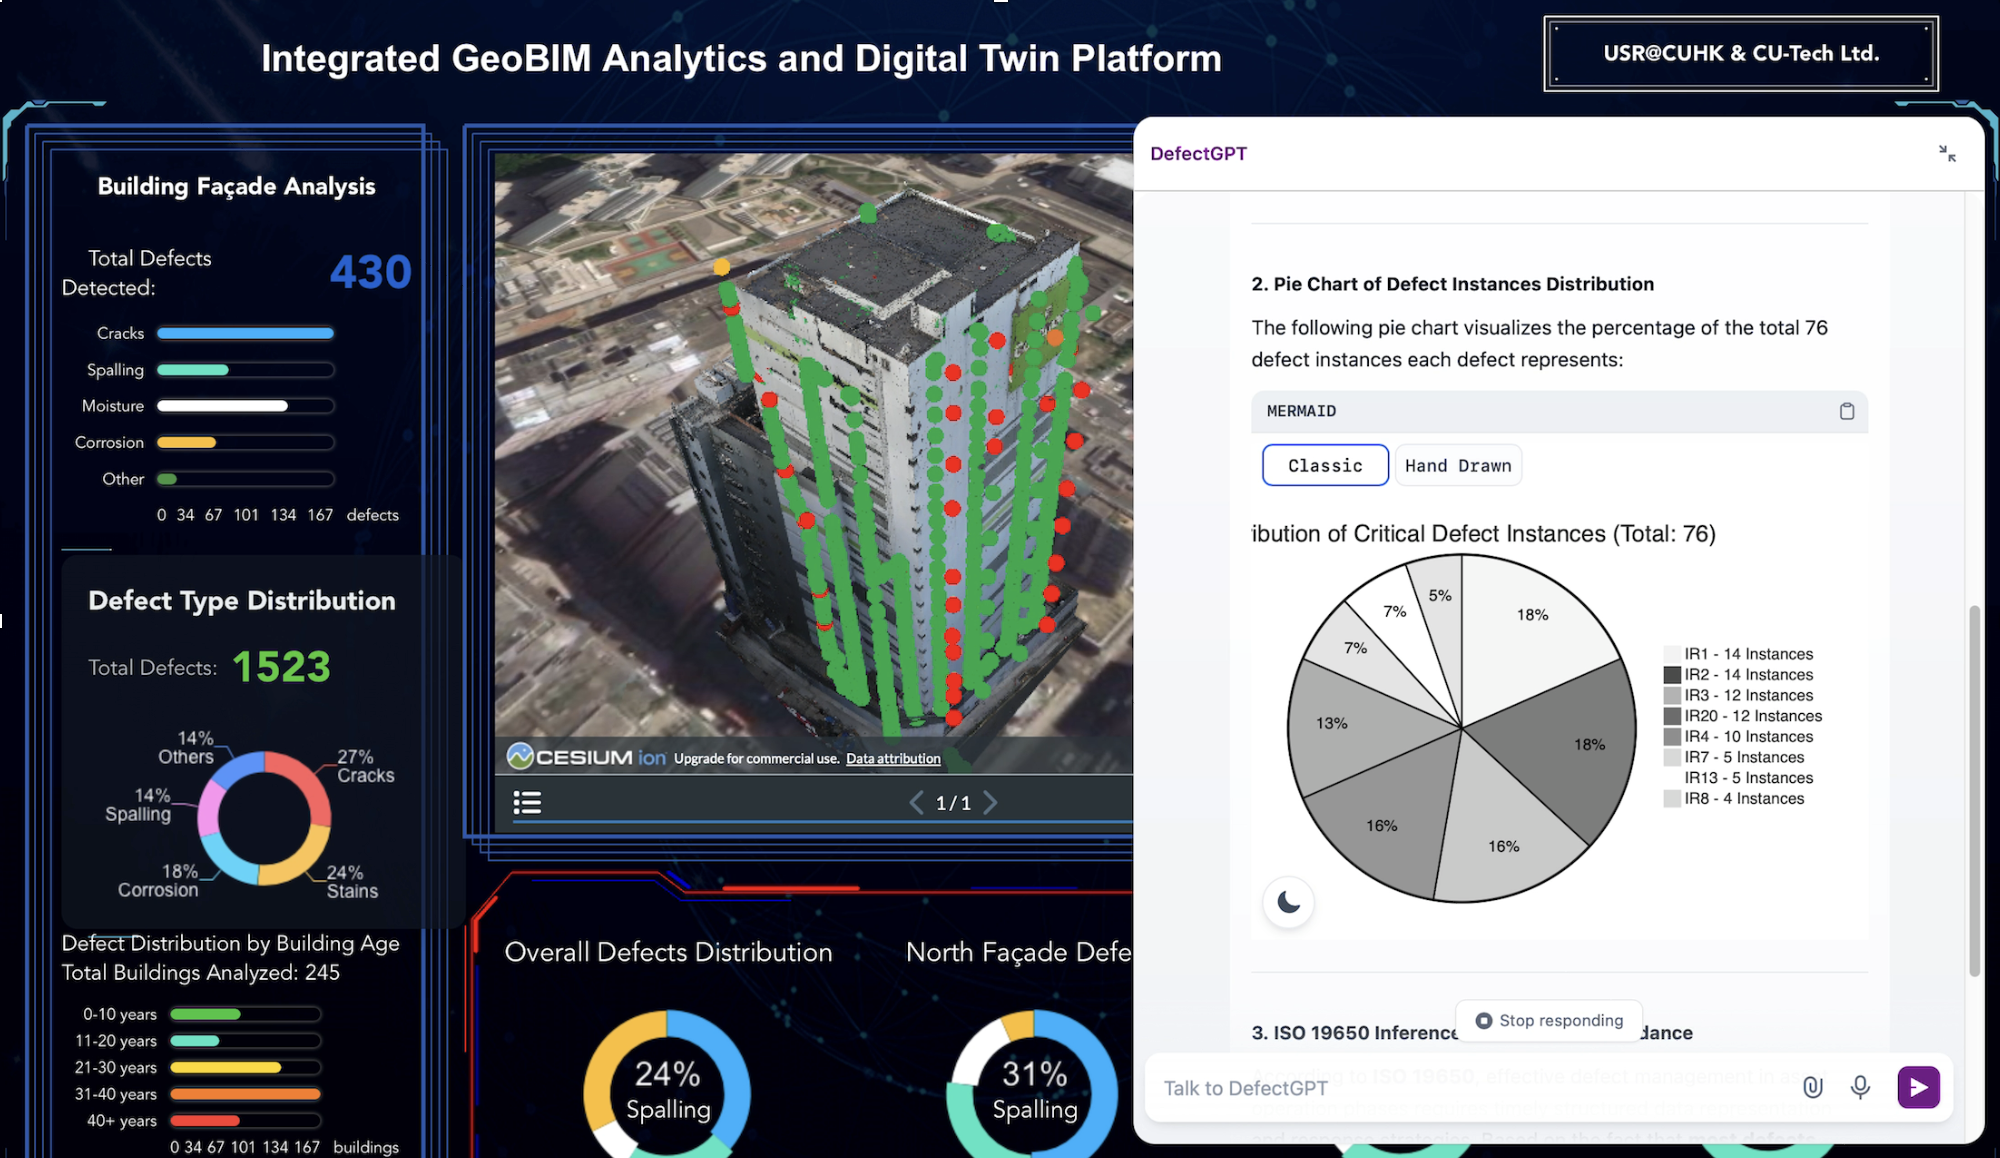
\includegraphics[width=0.9\textwidth]{figures/DefectGPT/System_implement.png}
\caption{CORTEX implementation for building health monitoring showing the integration of BIM data, IoT sensors, and diagnostic reasoning.}
\label{fig:system_implementation}
\end{figure}

The dataset construction process involves collaboration with building operators to identify representative diagnostic scenarios, expert annotation to establish ground truth labels and explanatory reasoning, data augmentation to ensure coverage of different fault types and building systems, and validation protocols to ensure dataset quality and reliability.

Each scenario includes complete Digital Twin data (BIM models, sensor readings, maintenance records, documentation), natural language problem descriptions that mirror real-world diagnostic requests, ground truth labels indicating correct diagnoses, expert explanations providing authoritative reasoning for comparison, and difficulty ratings based on complexity and required expertise level.

Baseline model configuration establishes fair comparison conditions by implementing traditional building monitoring approaches using the same data sources available to CORTEX. Baseline approaches include threshold-based alerting systems that flag sensor readings exceeding predefined limits, rule-based expert systems that encode diagnostic heuristics in formal rules, statistical anomaly detection methods that identify unusual patterns in sensor data, and human expert analysis using traditional tools and interfaces.

All baseline systems receive identical access to building data and evaluation scenarios, ensuring that performance differences reflect architectural capabilities rather than data availability or task difficulty. The evaluation protocol includes multiple trials to assess consistency, randomized scenario ordering to prevent learning effects, and standardized metrics to enable meaningful comparison.

Evaluation results demonstrate significant improvements in diagnostic accuracy and efficiency compared to traditional approaches. The CORTEX system achieved substantial reduction in false positive rates while maintaining high sensitivity for critical fault detection. Response accuracy showed notable improvement compared to both rule-based systems and threshold-based approaches. Time to diagnosis decreased considerably due to automated information synthesis and reasoning capabilities.

Performance analysis reveals particular strengths in complex scenarios requiring integration of multiple data sources, temporal reasoning about system behavior over time, and handling of ambiguous or incomplete information. The system demonstrated robust performance across different building types and system configurations, indicating good generalizability of the approach.

Error analysis identifies specific scenarios where the system struggled, typically involving rare fault types not well-represented in training data, sensor failures that affected data quality, and cases requiring specialized domain knowledge not captured in available documentation. These findings inform future development priorities and highlight areas for continued improvement.

\section{Summary of Findings}

The building health monitoring case study provides evidence for the L1 Descriptive Twin approach and demonstrates the potential effectiveness of DT-RAG for infrastructure applications. The research questions are addressed through systematic evaluation that shows clear benefits of cognitive enhancement over traditional approaches.

The architectural innovations developed for this case study provide reusable frameworks for similar infrastructure monitoring applications. Key innovations include multi-modal data fusion techniques that handle heterogeneous building data sources, temporal reasoning approaches that consider historical context and trends, and uncertainty quantification methods that provide reliable confidence estimates for diagnostic conclusions.

The DT-RAG architecture shows promise for handling the complex information integration requirements of modern building systems. The approach successfully bridges the gap between unstructured natural language queries and structured data sources while maintaining real-time responsiveness necessary for operational applications.

Current limitations include dependence on data quality and availability, challenges with rare or novel fault types not well-represented in historical data, and requirements for domain expertise in system configuration and validation. Future development should focus on improved handling of incomplete or corrupted data, enhanced learning from limited examples of rare faults, and automated approaches for system configuration and adaptation to new building types.

The findings establish a foundation for extending the approach to other infrastructure domains and provide insights for developing L2 Predictive Twin capabilities that build upon the information integration capabilities demonstrated in this case study.
